%
% Copyright (c) 2021 Antonio Coín Castro
%
% This work is licensed under a
% Creative Commons Attribution-ShareAlike 4.0 International License.
%
% You should have received a copy of the license along with this
% work. If not, see <http://creativecommons.org/licenses/by-sa/4.0/>.
%

\RequirePackage{fix-cm}
\documentclass[10pt, english, professionalfonts]{beamer}

\usepackage{pifont}  % xmark, cmark
\newcommand{\cmark}{\ding{51}}%
\newcommand{\xmark}{\ding{55}}%

% OPCIONES DE BEAMER

\definecolor{Maroon}{cmyk}{0, 0.87, 0.88, 0.1}
\definecolor{teal}{rgb}{0.0, 0.45, 0.45}

\usetheme[block=fill, subsectionpage=progressbar, titleformat section=smallcaps]{metropolis}
\setbeamertemplate{frametitle continuation}[roman]
\setbeamertemplate{section in toc}[sections numbered]
%\setbeamertemplate{subsection in toc}[subsections unnumbered]
%\setsansfont[BviejoFont={Fira Sans SemiBold}]{Fira Sans Book}  % Increase font weigth
\widowpenalties 1 10000
\raggedbottom

% COLORES
\setbeamercolor{palette primary}{bg=teal}
\setbeamercolor{progress bar}{use=Maroon, fg=Maroon}

% PAQUETES

\usepackage[utf8]{inputenc}
\usepackage[absolute,overlay]{textpos}
\usepackage[english]{babel}
\usepackage{microtype}
\usepackage{epigraph}
\usepackage{hyperref}
\usepackage{bm}
\usepackage{amssymb, amsmath, amsthm, amsfonts, amscd}
\usepackage{listings}

\usepackage[backend=biber,style=numeric-comp,sorting=none]{biblatex}
\addbibresource{bibliography.bib}
\setbeamertemplate{bibliography item}[article]

% FONTS
%\usefonttheme{professionalfonts}
%\usepackage{mathpazo}
%\usepackage{eulervm}

\definecolor{backg}{HTML}{F2F2F2} % Fondo
\definecolor{comments}{HTML}{a8a8a8} % Comentarios
\definecolor{keywords}{HTML}{08388c} % Palabras clave
\definecolor{strings}{HTML}{0489B1}  % Strings

\lstset{
language=scala,
basicstyle=\footnotesize\ttfamily,
breaklines=true,
keywordstyle=\color{keywords},
commentstyle=\color{comments},
stringstyle=\color{strings},
xleftmargin=.5cm,
tabsize=2,
% Acentos, ñ, ¿, ¡ (tex.stackexchange.com/questions/24528)
extendedchars=true
}

% COMANDOS PERSONALIZADOS


\renewcommand{\baselinestretch}{1}
\definecolor{mLightBrown}{HTML}{f97e0b}
\newcommand\maroon[1]{\color{mLightBrown}#1\color{mDarkTeal}}
\let\lmin\wedge
\let\lmax\vee
\newtheorem{prop}{Proposición}
\newtheorem{teorema}{Teorema}
\newtheorem{defi}{Definición}
\newcommand\ddfrac[2]{\frac{\displaystyle #1}{\displaystyle #2}}  % Fracción grande

\renewcommand{\epsilon}{\varepsilon}

\newcommand{\N}{\mathbb{N}}
\newcommand{\R}{\mathbb{R}}
\newcommand{\E}{\mathbb{E}}
\newcommand{\Hcal}{\ensuremath\mathcal{H}}

%% Scalar product
\newcommand\dotprod[2]{\left\langle #1, #2 \right\rangle}

% PLOTS

%\usepackage{pgfplots}
%\DeclareUnicodeCharacter{2212}{−}
%\usepgfplotslibrary{groupplots,dateplot}
%\usetikzlibrary{patterns,shapes.arrows}
%\pgfplotsset{compat=newest}

% TÍTULO

\title{Bayesian RKHS-based methods in functional regression}
\providecommand{\subtitle}[1]{}
\subtitle{Theoretical framework and experiments}
\date{SEIO Congress Granada\\ 8th May 2022\\}
\author{José R. Berrendero \\ Antonio Coín  \\ Antonio Cuevas\\}
\institute{Universidad Autónoma de Madrid \\ \textit{Departamento de Matemáticas}}

\titlegraphic{
  \begin{textblock*}{2cm}(9.8cm, 6.7cm)
    
\includegraphics[width=2cm]{img/logo-uam}
  \end{textblock*}
}
% DOCUMENTO

\begin{document}
\maketitle

\begin{frame}{Table of contents}
  \tableofcontents
\end{frame}

\section{Introduction}

\begin{frame}{FDA: linear regression}
  \textbf{First problem}: \maroon{Linear } regression with functional data.
  \vspace{1em}

\begin{figure}
    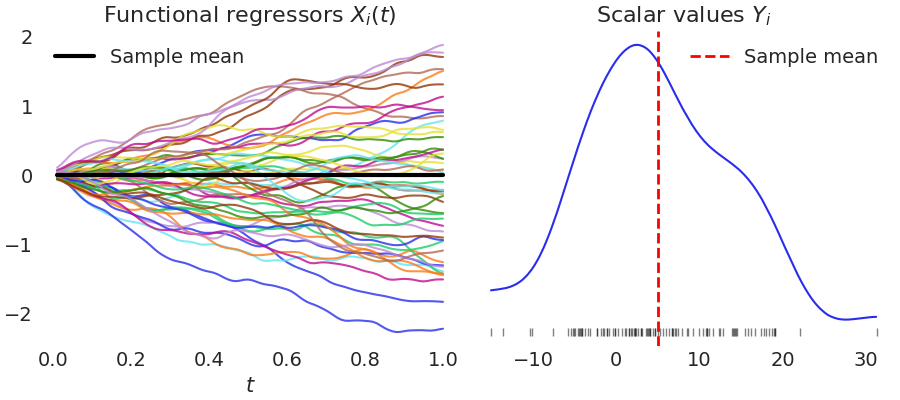
\includegraphics[width=\textwidth]{img/data_lin}
    \caption{Linear regression data set simulated from a fractional brownian motion.}
  \end{figure}
  \vspace{-1em}
\end{frame}
\begin{frame}{FDA: logistic regression}
  \textbf{Second problem}: \maroon{Logistic } regression with functional data.
\vspace{1em}

\begin{figure}
    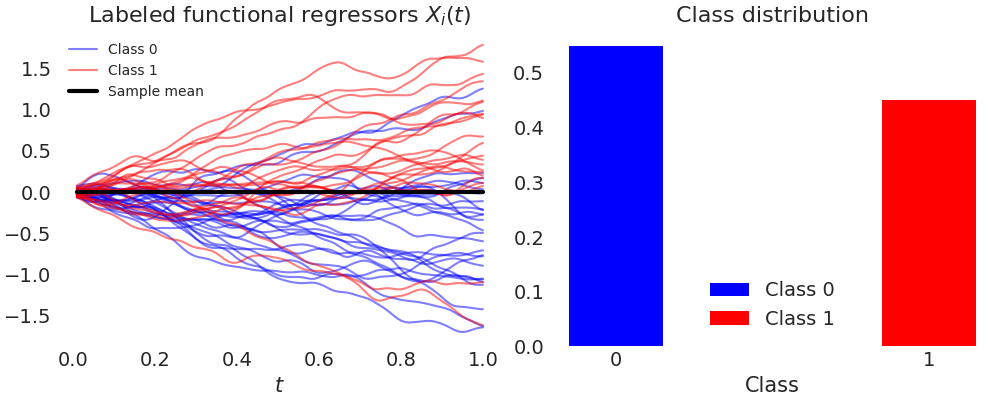
\includegraphics[width=\textwidth]{img/data_log}
    \caption{Logistic regression data set simulated from a fractional brownian motion.}
  \end{figure}
  \vspace{-1em}
\end{frame}

\begin{frame}{The usual \(\bm{L^2}\)-models}
  \(\bullet\) \(Y\) real variable (continuous or dichotomous).

  \(\bullet\) \(X(t)\) second order stochastic process with trajectories in \(L^2[0, 1]\).

  \(\bullet\) \(\beta \in L^2[0,1]\) \maroon{functional parameter}.

  \vspace{1em}

\begin{block}{Linear \(\bm{L^2}\)-model}
  \[
    Y = \alpha_0 + \maroon{\langle X, \beta \rangle_2} + \varepsilon = \alpha_0 + \int_0^1 X(t)\beta(t)\, dt + \varepsilon.
  \]
\end{block}
\begin{block}{Logistic \(\bm{L^2}\)-model}
    \[
    \mathbb P (Y=1\mid X) = \frac{1}{1 + \exp\{-\alpha_0 - \maroon{\langle X, \beta\rangle_2}\}} = \frac{1}{1 + \exp\{-\alpha_0 - \int_0^1 X\beta\}}.
  \]
\end{block}
  \(\alpha_0\in\mathbb R\), \ \(\varepsilon \sim \mathcal N(0, \sigma^2), \ \mathbb E[\varepsilon]=0, \ X \bot \varepsilon\).
\end{frame}


\begin{frame}{Shortcomings of the \(\bm{L^2}\)-models}
  \begin{itemize}
    \item \(L^2[0, 1]\) is a extremely wide space, which also contains very ill-behaved functions.
    \item The usual least-squares theory cannot be applied directly; some regularization or dimensionality reduction techniques are required.
    \item They do not include simple models based on linear combinations of the marginal of the process as particular cases, such as
    \[
      Y = \alpha_0 + \sum_{j=1}^p \beta_j X(t_j) + \varepsilon.
    \]
    \item In the logistic case, the maximum likelihood estimator does not exist with probability one under fairly general conditions.
  \end{itemize}
\end{frame}

\section{A RKHS model for functional regression}


\begin{frame}{Alternative model: RKHS}

We will exploit the theory of \textit{reproducing kernel Hilbert spaces} (RKHS's).

\vspace{1em}
\begin{alertblock}{Proposal}
  Change the habitat of the functional parameter \(\beta(\cdot)\).
\end{alertblock}

\vspace{1em}
  Instead of assuming \(\beta \in L^2[0, 1]\), we consider \maroon{\(\beta \in \mathcal H(K)\)}, the RKHS associated with the covariance function \(K(t, s)=\mathbb E[X(t)X(s)]\) of the centered process \(X\). Moreover, we substitute \(\dotprod{X}{\beta}_2\) for \maroon{\(\dotprod{X}{\beta}_K\)}.
\end{frame}


\begin{frame}{RKHS reminder}
  \begin{definition}
    Let \(K\) be continuous, and define the preliminary space
    \[
    \Hcal_0(K) = \left\{ f \in L^2[0,1]: \ f(\cdot) = \sum_{i=1}^p a_i K(t_i, \cdot),  p \in \N,  a_i \in \R,  t_i \in [0, 1] \right\},
    \]
    which is endowed with the scalar product \(\dotprod{f}{g}_K = \sum_{i, j} a_i b_j K(t_i, s_j)\), for \(f(\cdot)=\sum_i a_i K(t_i, \cdot) \) and \(g(\cdot)=\sum_j b_j K(s_j, \cdot)\). Then, \(\Hcal(K)\) is the completion of \(\Hcal_0(K)\) under this scalar product.
  \end{definition}

  \vspace{1em}

  Note that \(\Hcal(K)\subset L^2[0, 1]\), but the elements of \(\Hcal(K)\) are simpler and more manageable in general. Plus, the latter is a space of \maroon{functions}, and not of equivalence classes.
\end{frame}


% \begin{frame}{Un repaso muy breve de los RKHS's (cont.)}
% Se pueden dar otras definiciones equivalentes de \(\Hcal(K)\), basadas en el \textit{operador de covarianzas}
% \[
% \mathcal Kf(\cdot) = \int_0^1 K(s, \cdot)f(s)\, ds, \quad f\in L^2[0, 1].
% \]
%
% \begin{definition}
% \begin{enumerate}
%   \item  \(\Hcal(K) = \mathcal K^{1/2}(L^2[0, 1])\), con \(\dotprod{f}{g}_K = \dotprod{\mathcal K^{-1/2}(f)}{\mathcal K^{-1/2}(g)}_2\).
%   \item \(\Hcal(K) = \{f \in L^2[0, 1]: \ \sum_j \lambda_j^{-1}\dotprod{f}{\phi_j}^2 < \infty \}\), con \(\dotprod{f}{g}_K = \sum_j \lambda_j^{-1}\dotprod{f}{\phi_j}\dotprod{g}{\phi_j}_2\). En este caso, \(\lambda_j\) y \(\phi_j\) son los autovalores y autofunciones de \(\mathcal K\).
% \end{enumerate}
% \end{definition}
%
% La segunda de estas definiciones enfatiza el hecho de que las funciones de \(\Hcal(K)\) son ``simples'', en el sentido de que sus componentes en una base ortonormal tienden a \(0\) rápidamente.
%
% \end{frame}

\begin{frame}{A small subtlety}

  Generally speaking, the concrete realizations \(x=X(\omega)\) \maroon{do not belong to \(\Hcal(K)\) with probability \(1\)}, so the expression \(\dotprod{x}{\beta}_K\) lacks meaning. However, we can make use of the relationship between \(\Hcal(K)\) and \(\mathcal L(X)\), the linear span of the process \(X\) within \(L^2(\Omega)\).


  \vspace{1em}
  \begin{block}{Loève's isometry}
    It is the completion of the correspondence
    \[
\sum_{j=1}^p a_j X(t_j) \longleftrightarrow \sum_{j=1}^p a_j K(t_j, \cdot).
    \]
    Formally, \(\Psi^{-1}_X(U)(t) := \E[U X(t)]\) for \(U \in \mathcal L(X)\).
  \end{block}
  With a slight abuse of notation, we will write \maroon{\(\dotprod{x}{\beta}_k \equiv \Psi_x(\beta)\)}. This correspondence will allow us to still call our models ``linear''.
\end{frame}


\begin{frame}{A new functional parameter...}
  \begin{itemize}
    \item The initial idea was to suppose \(\beta \in \Hcal(K)\).
    \item To further simplify the model, we will assume \(\beta \in \Hcal_0(K)\), which is dense in \(\Hcal(K)\) by construction. That is,
    \[
      \beta(\cdot) = \sum_{j=1}^p \beta_j K(t_j, \cdot).
    \]
    \item When evaluating \(\dotprod{x}{\beta}_K\) for a trajectory \(x=X(\omega)\), we resort to Loeve's isometry:
    \[
      \dotprod{x}{\beta}_K = \Psi_x(\beta) = \sum_{j=1}^p \beta_j X(t_j).
    \]
  \end{itemize}

\end{frame}


\begin{frame}{...and two new models}
  Given a data set \(\mathcal D_n = \{(X_i, Y_i): i=1,\dots, n\}\) composed of i.i.d. samples of \((X, Y)\), we consider:

  \vspace{1em}

  \begin{block}{Linear RKHS model (Berrendero et al., 2019)}
  \[
    Y_i = \alpha_0 + \maroon{\langle X_i, \beta \rangle_K} + \varepsilon = \alpha_0 + \sum_{j=1}^p \beta_j X_i(t_j) + \varepsilon.
  \]
\end{block}
\vspace{1em}
\begin{block}{Logistic RKHS model (Berrendero et al., 2018)}
    \[
    \mathbb P (Y_i=1\mid X_i) = \frac{1}{\exp\{-\alpha_0 - \maroon{\langle X_i, \beta\rangle_K}\}} = \frac{1}{\exp\{-\alpha_0 - \sum_{j=1}^p \beta_j X_i(t_j)\}}.
  \]
\end{block}

\end{frame}

\section{A bayesian approach to parameter estimation}

\begin{frame}{Parameter estimation overview}

  We have a parameter vector \(\theta = (p, \beta_1,\dots, \beta_p, t_1,\dots, t_p, \alpha_0, \sigma^2)\), on which we impose a prior distribution \(\pi(\theta)\). In practice, we are establishing a prior distribution on the functional space \(\Hcal(K)\) via a density argument.

  \vspace{1em}

  Afterwards we apply \textit{Bayes'}  theorem in the usual way to obtain the posterior distribution of the parameters given the data.

  \begin{block}{Bayes's theorem}
      \[
      \pi(\theta \mid \mathcal D_n) \propto \left( \prod_{i=1}^n \pi(Y_i\mid X_i, \theta) \right)\pi(\theta).
      \]
  \end{block}
  \vspace{1em}

  Finally, we obtain samples of the approximate posterior distribution using an algorithm of the family of \textit{Markov chain Monte Carlo} (MCMC) methods.

\end{frame}

\begin{frame}{Prior distributions}
  Same prior scenario for both linear and logistic models.
  \begin{block}{Prior for the parameters involved}
    \vspace{-1em}
  \begin{align*}
    p &\sim \text{Categorical}(p_{\text{max}}),\\
  \pi(\alpha_0, \sigma^2)              & \propto 1/\sigma^2,                                                     \\
  \tau                     & \sim \mathcal U([0, 1]^p),                                              \\
  \beta\mid \tau, \sigma^2 & \sim \mathcal N\big(b_0, g\sigma^2{\underbrace{\left[\mathcal X_\tau' \mathcal X_\tau + \eta I\right]}_{G_\tau}}^{-1}\big),
\end{align*}
where \(I\) is the identity matrix, \(\mathcal X_\tau = (X_i(t_j))_{i,j}\), and \(b_0\in \R^p, \ g \in \R, \ p_{\text{max}}\in \N\) and \(\eta \in \R^+\) are hyperparameters.
\end{block}

\metroset{block=transparent}

\begin{alertblock}{Hyperparameter selection}
  \vspace{0.1em}
  For \(b_0\) we use a computational approximation of the MLE; the rest of hyperparameters are set via \textit{cross-validation}.
\end{alertblock}
\metroset{block=fill}
\end{frame}

\begin{frame}{Posterior distributions}
  \begin{block}{Linear log-posterior}
    \vspace{-1em}
    \begin{align*}
  \log \pi(\theta\mid \mathcal D_n) &\propto \frac{1}{2}\log |G_\tau| - (p+n)\log \sigma\\
  &-\frac{1}{2\sigma^2} \left(\|\boldsymbol{Y}-\alpha_0\boldsymbol{1} - \mathcal X_\tau\beta\|^2 + \frac{1}{g}(\beta - b_0)'G_\tau(\beta - b_0) \right),
\end{align*}
where \(\bm Y=(Y_1,\dots,Y_n)'\) y \(\bm{1}\) is an \(n\)-dimensional vector of ones.
  \end{block}

\vspace{1em}
  \begin{block}{Logistic log-posterior}
      \vspace{-1em}
    \begin{align*}
  \log \pi(\theta \mid \mathcal D_n) \propto {} & \sum_{i=1}^n \left[ \left(\alpha_0 + \Psi_{X_i}(\alpha)\right)Y_i - \log\left(1 + \exp\left\{\alpha_0 + \Psi_{X_i}(\alpha)\right\}\right)\right]\\
  \quad &+ \frac{1}{2}\log |G_\tau| - p\log \sigma -\frac{1}{2g\sigma^2} (b - b_0)'G_\tau(b - b_0).
\end{align*}
Remember that \(\Psi_{X_i}(\alpha) = \sum_j \beta_j X_i(t_j)\).
  \end{block}
\end{frame}

\begin{frame}{Posterior approximation}
  We use the Python library \maroon{emcee}, which implements an MCMC algorithm consisting on multiple chains that interact with each other to advance on each step (\textit{Affine-invariant ensemble sampler}).

  \vspace{1em}

  \begin{figure}
    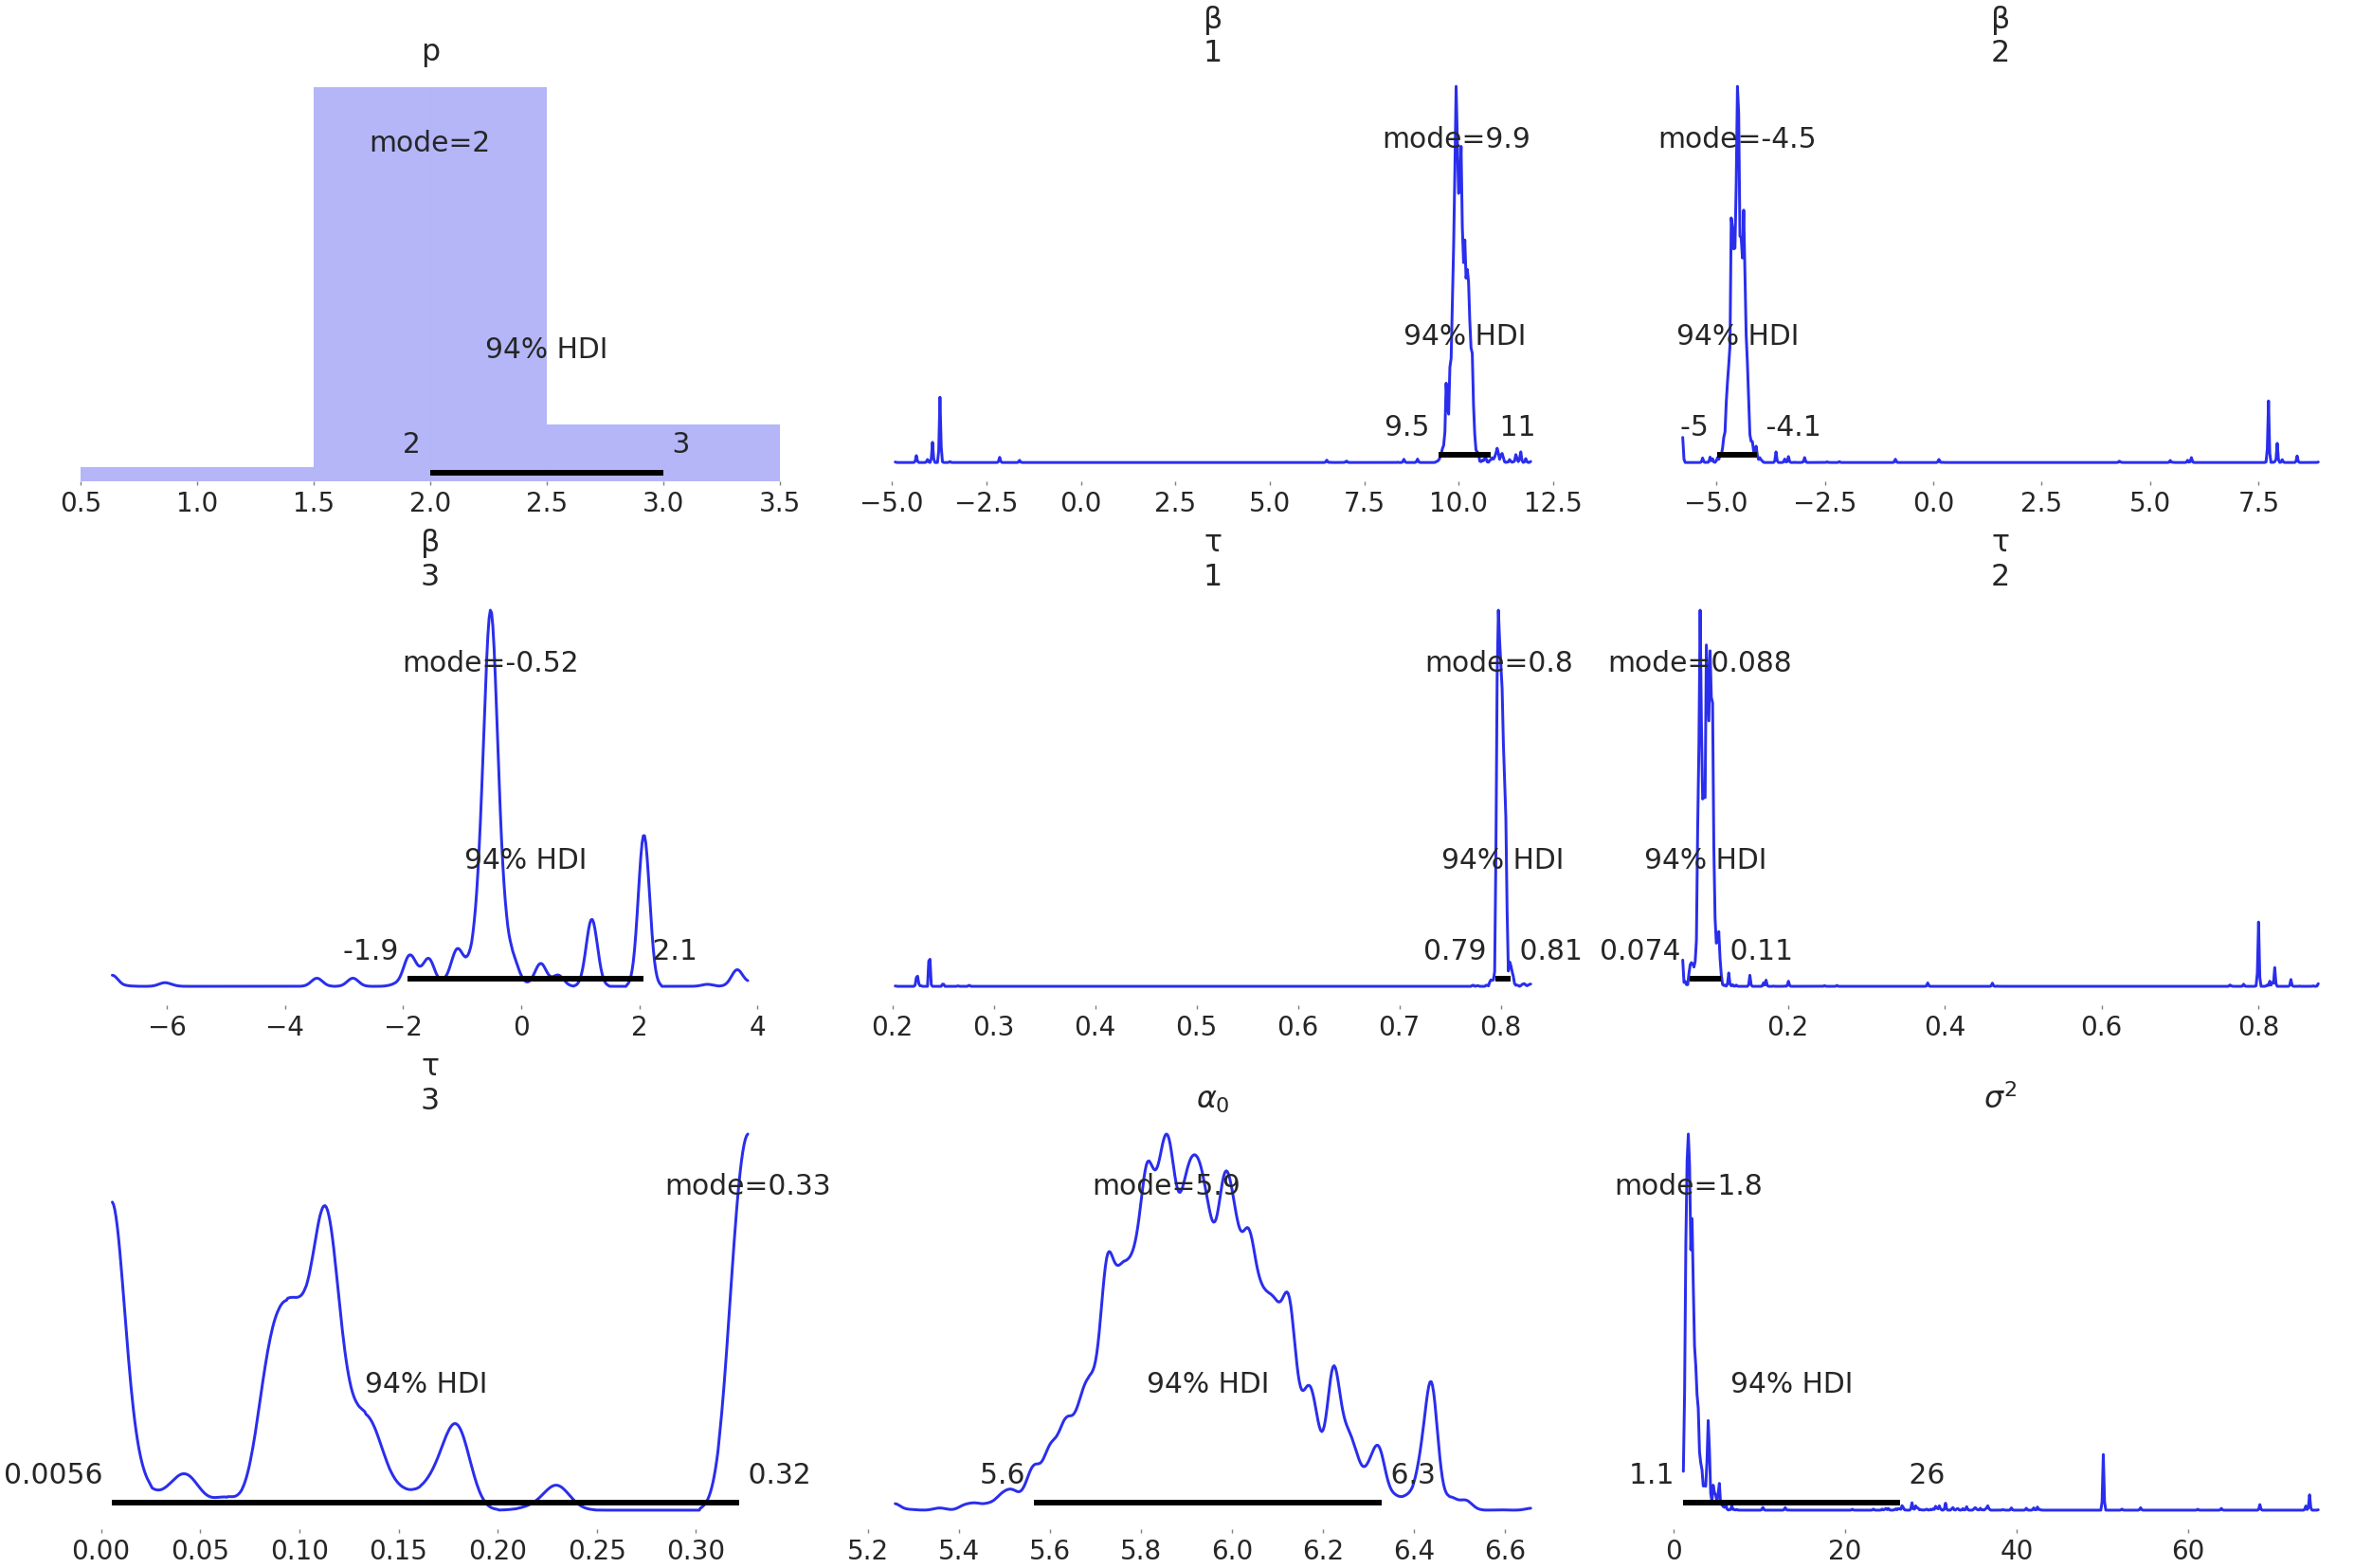
\includegraphics[width=.7\textwidth]{img/posterior}
    \caption{Example of an approximated posterior distribution \(\theta|\mathcal D_n\).}
  \end{figure}
\end{frame}

\begin{frame}{Predictions}
  \textbf{Summarize-then-predict}. A summary of the posterior distribution \(\theta| \mathcal D_n\) is obtained via a point-estimate statistic (mean, median, mode), and then predictions are made according to the assumed model, e.g.:
  \[
  \hat Y_i =\hat \alpha_0 + \sum_{j=1}^p \hat \beta_j X_i(\hat \tau_j), \quad i=1,\dots, n.
  \]

  \textbf{Predict-then-summarize}. For each MCMC iteration we get a sample \(\theta^{(m)*}\) of the approximate posterior. We first construct predictions on each step following our model, i.e.:
  \[
    Y_i^{(m)*} \equiv Y_i \mid X_i, \theta^{(m)*}, \quad m=1,\dots,M, \quad i=1,\dots, n.
  \]

  Then, the mean of all such intermediate predictions (\textit{posterior predictive distribution}) is used as a proxy for the response variable:
  \[
    \hat Y_i = \frac{1}{M}\sum_{m=1}^M Y_i^{(m)*}, \quad i=1,\dots, n.
  \]

\end{frame}

\begin{frame}{Predictions (cont.)}
    \textbf{Variable selection}. We select \(p\) variables using only a point estimator of \(\tau=(t_1,\dots, t_p)|\mathcal D_n\) (so-called \textit{impact points}), and then we can apply any multiple regression algorithm to the reduced data set.
    \vspace{1em}

    \begin{figure}
      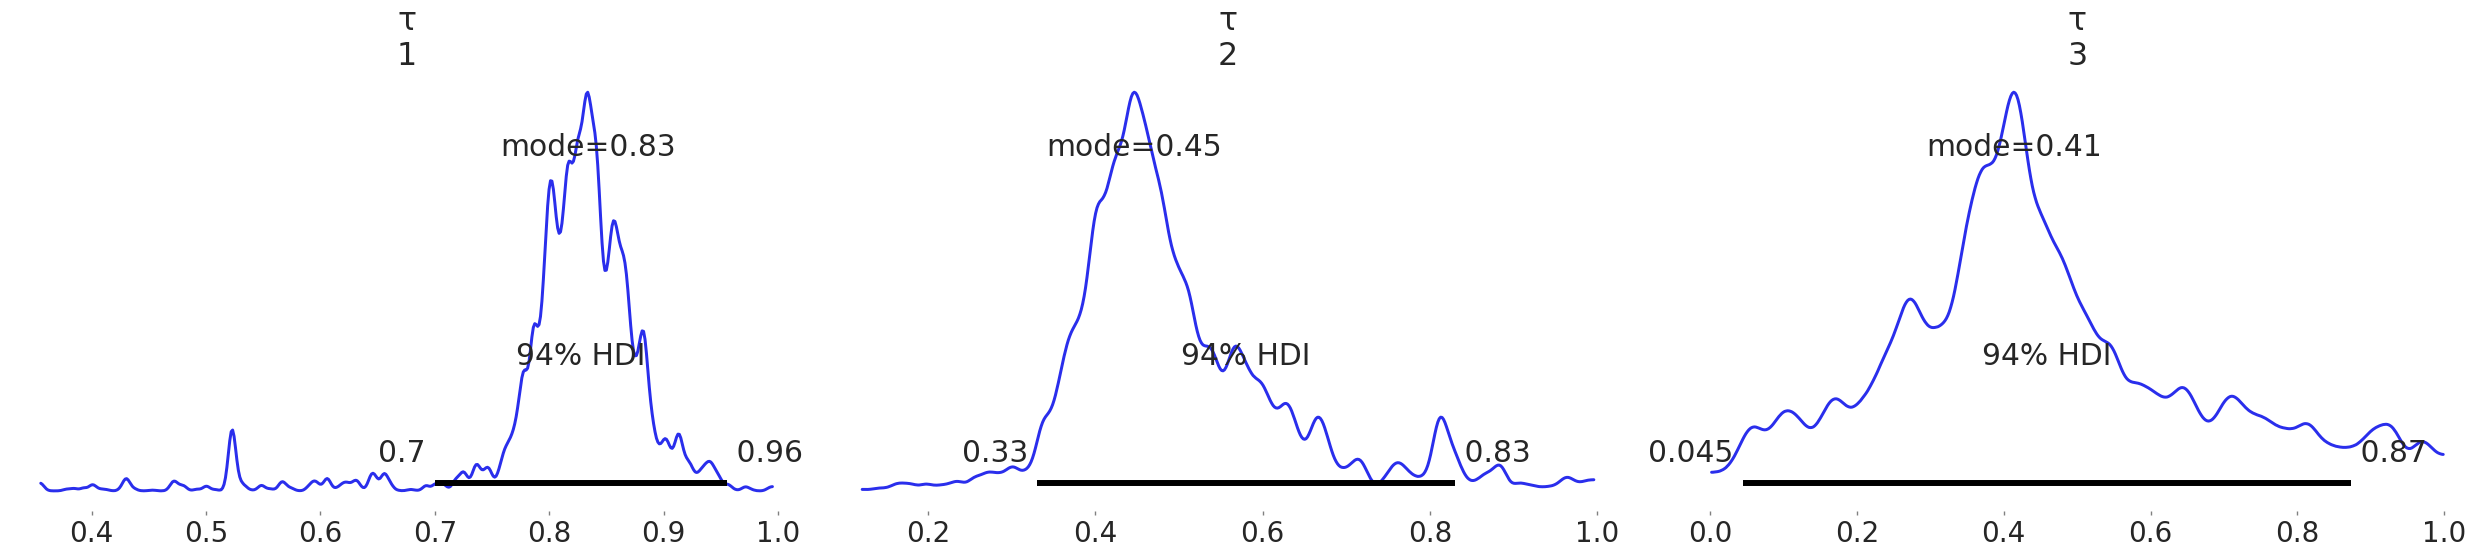
\includegraphics[width=\textwidth]{img/tau_posterior}
      \caption{Approximate posterior distribution for the impact points.}
    \end{figure}

    At any rate, all the above predictors can be obtained after a single run of the MCMC algorithm.
\end{frame}

\begin{frame}{Model checking}
  \begin{itemize}
    \item Analysis of the trace and posterior distribution of the parameters, for example through credible intervals.
    \item \textit{Bayesian p-values}: \(\tilde p=P(T(Y^*)\leq T(Y)\mid Y)\) for any choice of \(T\): min, max, mean, median, mode, etc. They are computed by simply measuring the proportion of the approximate posterior samples that fall below the real value of the statistic, and are expected to be around \(0.5\) when the fit is good.
    \item Descriptive and visual analysis of the posterior predictive distribution, both with training and validation data.
  \end{itemize}

\end{frame}

\begin{frame}{Model checking (cont.)}
  \begin{figure}
    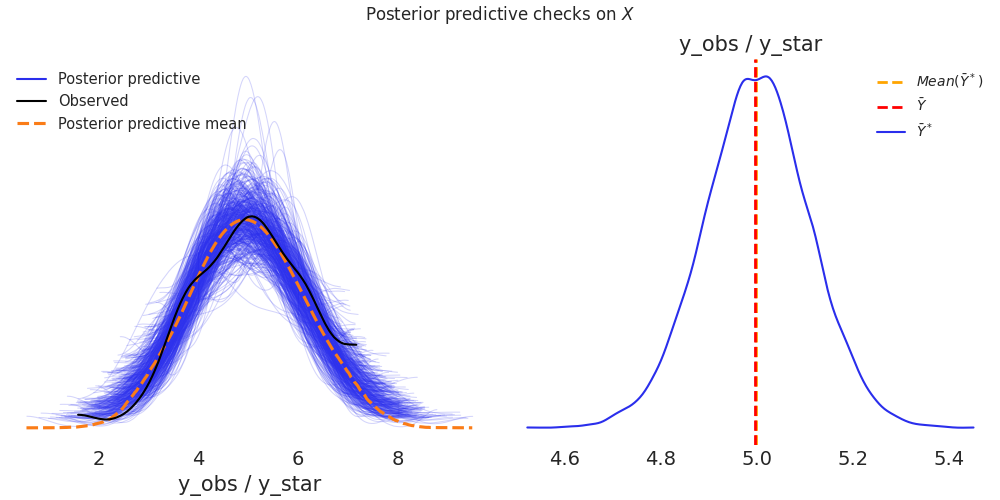
\includegraphics[width=\textwidth]{img/ppc_linear}
    \caption{\textit{Posterior predictive checks} for linear regression.}
  \end{figure}
\end{frame}

\begin{frame}{Model checking (cont.)}
  \begin{figure}
    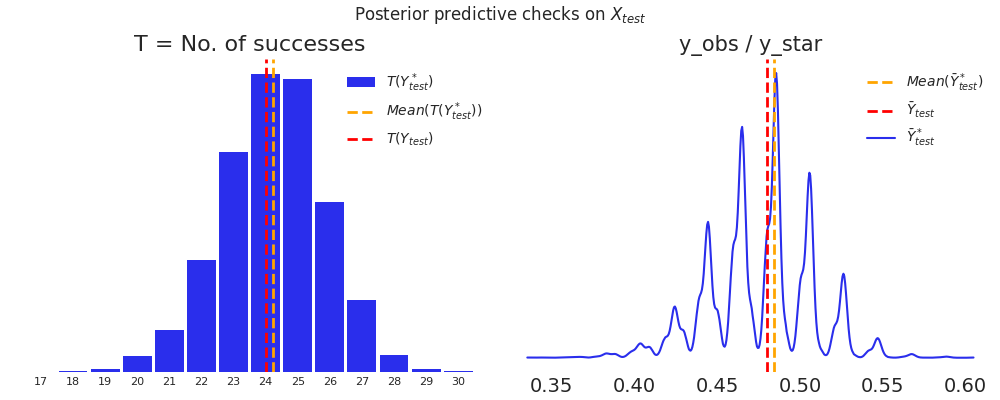
\includegraphics[width=\textwidth]{img/ppc_logistic1}
    
\includegraphics[width=\textwidth]{img/ppc_logistic2}
    \caption{\textit{Posterior predictive checks} for logistic regression.}
  \end{figure}
\end{frame}

\section{Experiments}

\begin{frame}{Methodology}
  \begin{itemize}
    \item Experiments on simulated data, with \(150\) samples of different Gaussian processes on a regular grid of \(100\) points. Also on real data sets.
    \item We perform 10 random train/test partitions to account for the stochasticity of the model, along with \(5\)-fold cross-validation to select the best hyperparameters on the training set.
    \item For practical and computational reasons, \textbf{we allow the value of \(\bm{p}\) to be fixed beforehand}, treating it as an hyperparameter (equivalent to a degenerate prior distribution). {\color{red} problema de indentificabilidad de coeficientes!!}
    \item Several functional reference algorithms for comparison, along with variable selection techniques, functional or otherwise.

  \end{itemize}
\end{frame}

\begin{frame}{Linear regression: simulated data}
  \vspace{1em}
  \begin{figure}
    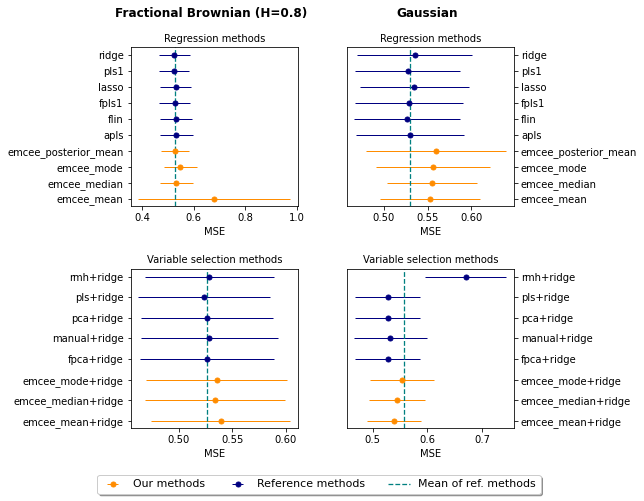
\includegraphics[width=\textwidth]{img/reg_emcee_l2}
    \caption{Mean MSE of predictors for simulated data that has an underlying \(L^2\)-model.}
  \end{figure}
\end{frame}

\begin{frame}{Linear regression: simulated data}
    \vspace{1em}
  \begin{figure}
    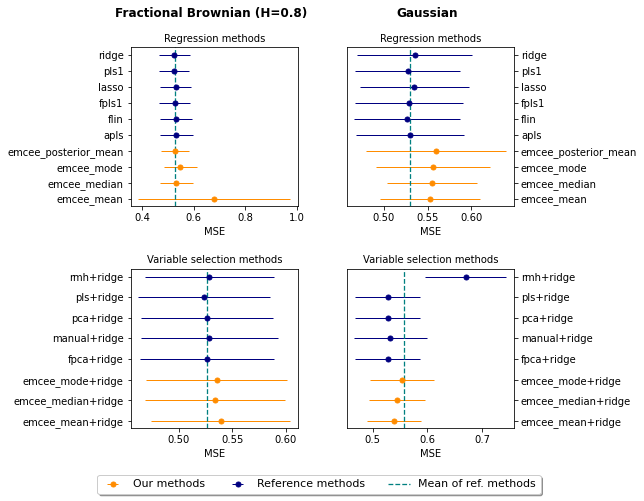
\includegraphics[width=\textwidth]{img/reg_emcee_l2}
    \caption{Mean MSE of predictors for real data sets.}
  \end{figure}
\end{frame}

\begin{frame}{Logistic regression: simulated data}
    \vspace{1em}
  \begin{figure}
    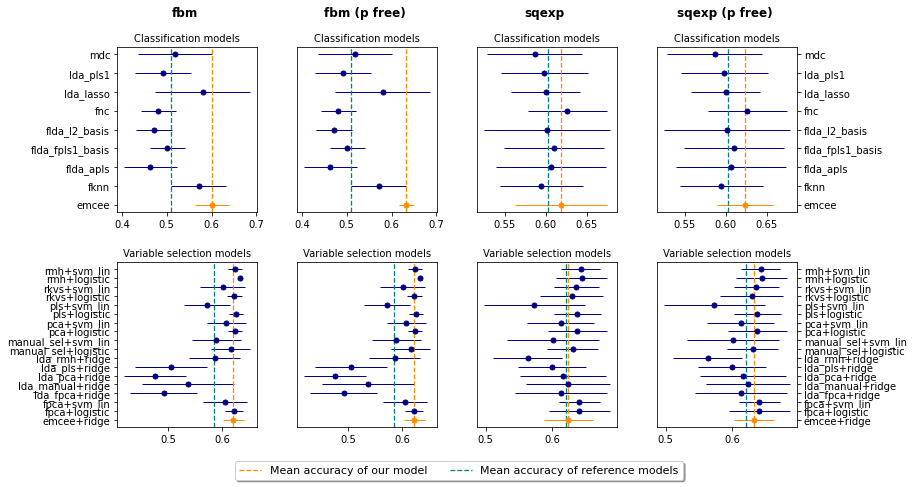
\includegraphics[width=\textwidth]{img/clf_emcee_l2}
    \caption{Mean accuracy of classifiers for simulated data that has an underlying logistic \(L^2\)-model.}
  \end{figure}
\end{frame}

\begin{frame}{Logistic regression: real data}
    \vspace{1em}
  \begin{figure}
    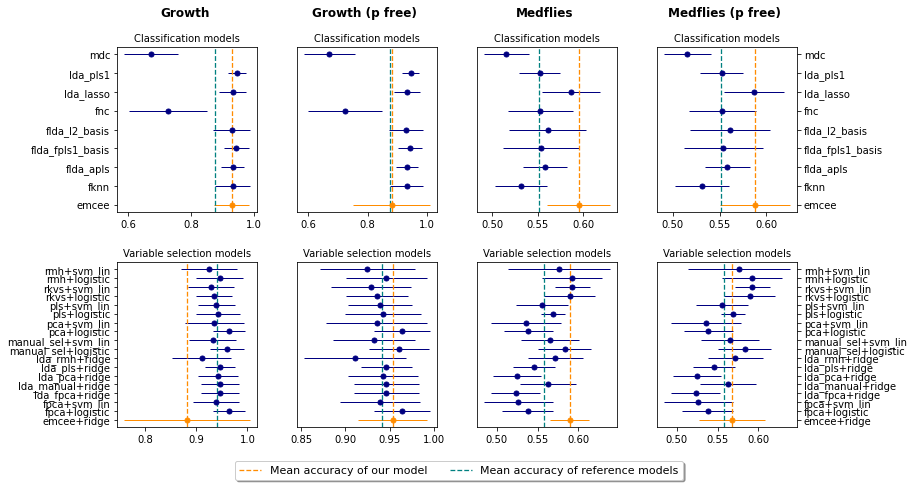
\includegraphics[width=\textwidth]{img/clf_emcee_real}
    \caption{Mean accuracy of classifiers for real data sets.}
  \end{figure}
\end{frame}

\begin{frame}{Conclusions and future work}

  \metroset{block=transparent}
  \begin{alertblock}{Our proposal}
    \begin{itemize}
      \item Simple model for functional regression, with a solid mathematical background thanks to the theory of RKHS's.
      \item Computationally feasible Bayesian approach to parameter estimation within the model.
      \item Competitive with usual alternatives in both simulated and real data sets.
    \end{itemize}
  \end{alertblock}

  \begin{exampleblock}{The road ahead}
    \begin{itemize}
      \item Choose other prior distributions.
      \item Package the algorithm and make it compatible with standard libraries (e.g. \textit{sklearn}).
      \item Reduce the variance in predictions, possibly by tackling the \textit{label switching} problem.
    \end{itemize}
  \end{exampleblock}


\end{frame}

\begin{frame}[allowframebreaks]
    \frametitle{References}
    \nocite{*}
    \printbibliography[heading=none]
\end{frame}

\begin{frame}[standout]
  Thank you!
\end{frame}


\end{document}
